\documentclass{article}
\usepackage[utf8]{inputenc}
\usepackage[T1]{fontenc}
\usepackage{amsmath}
\usepackage{xcolor}
\usepackage{amssymb}
\usepackage{pgfplots}
\usepackage{pgfplotstable}
\pgfplotsset{compat=1.7}
\usepackage{tikz}
\usetikzlibrary{positioning}
\usetikzlibrary{arrows}
\usepgfplotslibrary{fillbetween}

\begin{document}

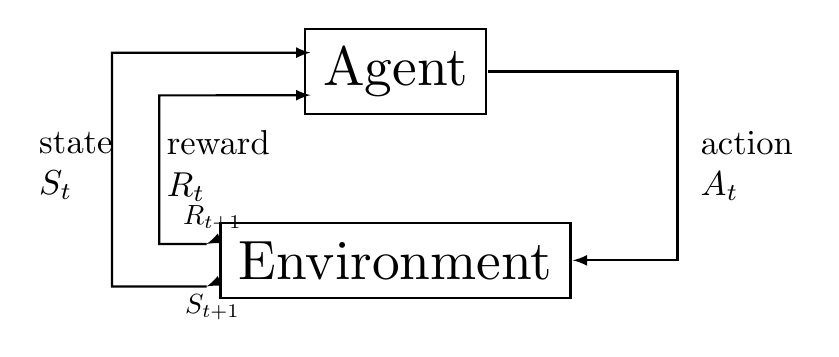
\begin{tikzpicture}[scale=0.6]

  \node[rectangle,draw,scale=2,thick] (agent) {Agent};
  \node[rectangle,draw,below=8.75ex of agent, scale=2,thick] (environment) {Environment};

  \draw[dotted,scale=2,thick] -- (-2,-1.7) -- (-2,-2.4);

  \draw [-{latex},scale=2,thick] 
    (agent.east) -- +(2,0) |-  (environment);
  \node[scale=1.25,text width=1cm] at (7.5,-2) {action $A_t$};

  \draw [-{latex},scale=2,thick] 
    (environment.west)+(0,0.225) -- node[above] {$R_{t+1}$} (-2,-1.825);

  \draw [-{latex},scale=2,thick] 
    (environment.west)+(0,-0.225) -- node[below] {$S_{t+1}$} (-2,-2.275);

  \draw [-{latex},scale=2,thick] 
    (-2,-1.825) |- +(-.5,0) |- +(0,1.5725) -- (-.9,-0.25);
  \node[scale=1.25, text width=1cm] at (-3.8,-2) {reward $R_t$};    

  \draw [-{latex},scale=2,thick] 
    (-2,-2.275) |- +(-1,0) |- +(0,2.4725) -- (-.9,0.2);
  \node[scale=1.25, text width=1cm] at (-6.5,-2) {state $S_t$};
\end{tikzpicture}

\end{document}